%% Passagem de opções para pacotes
\PassOptionsToPackage{english, main = brazilian}{babel}%% Suporte multilíngue

%% Classe e opções de documento
\documentclass[
  article,            %% Tipo de documento
  11pt,               %% Tamanho de fonte exigido
  letterpaper,        %% Tamanho de papel exigido (Letter)
  oneside,            %% Impressão anverso
  sumario = tradicional
]{abntex2}


%% Pacotes de Idioma e Codificação
\usepackage[utf8]{inputenc}
\usepackage[english]{babel}

%% Pacote de Estilo Customizado (Requer o arquivo .sty no Overleaf)
\usepackage{utfprpgtex-article} 

% --- 1. Eliminar a barra '/' e limpar o cabeçalho do topo ---
% Redefinimos os comandos internos do .sty para que fiquem vazios
\renewcommand{\lutfprheader}{}
\renewcommand{\rutfprheader}{}

% Configuramos o estilo de página para garantir que o topo está limpo e o número está em baixo
\makepagestyle{articlestyle}
\makeevenhead{articlestyle}{}{}{}
\makeoddhead{articlestyle}{}{}{}
\makeevenfoot{articlestyle}{}{}{\footnotesize\sffamily\thepage}
\makeoddfoot{articlestyle}{}{}{\footnotesize\sffamily\thepage}

% Removemos as linhas horizontais que o modelo UTFPR coloca no topo
\makeheadrule{articlestyle}{0pt}{0pt}

% --- 2. Centralizar os títulos de todas as secções ---
% Utilizamos os comandos da classe memoir (base do abntex2) para alinhar ao centro
\setsecheadstyle{\centering\ABNTEXsectionfont\ABNTEXsectionfontsize}
\setsubsecheadstyle{\centering\ABNTEXsubsectionfont\ABNTEXsubsectionfontsize}
\setsubsubsecheadstyle{\centering\ABNTEXsubsubsectionfont\ABNTEXsubsubsectionfontsize}

% --- Configuração para mover o número da página para o rodapé ---
\makepagestyle{articlestyle}
\makeevenhead{articlestyle}{\lutfprheader}{}{} % Limpa o topo direito
\makeoddhead{articlestyle}{\lutfprheader}{}{}  % Limpa o topo direito
\makeevenfoot{articlestyle}{}{}{\footnotesize\sffamily\thepage} % Adiciona embaixo à direita
\makeoddfoot{articlestyle}{}{}{\footnotesize\sffamily\thepage}  % Adiciona embaixo à direita
% ---------------------------------------------------------------

%% Pacotes Matemáticos e Técnicos
\usepackage{amsmath, amsthm, amssymb, amsfonts}
\usepackage{mathtools, bm, dsfont}
\usepackage{algorithm} 
\usepackage{algpseudocode} 
\usepackage{enumerate}

%% Pacotes de Elementos Visuais
\usepackage{graphicx}
\usepackage{booktabs, array, multirow}
\usepackage{caption}
\usepackage[section]{placeins}
\usepackage[many]{tcolorbox}
\usepackage{xcolor}
\graphicspath{ {./Figuras/} }

%% TikZ — diagramas de pipeline e dependências de módulos
\usepackage{tikz}
\usetikzlibrary{arrows.meta, shapes.geometric, positioning, fit, calc, backgrounds}

%% Coluna de largura fixa em tabelas
\usepackage{tabularx}

%% Referências e Hiperlinks
\usepackage[colorlinks=true, allcolors=blue]{hyperref}
\usepackage{url}
% REMOVIDO: \usepackage{natbib} para evitar conflito com o biblatex do .sty

\hypersetup{
    citecolor=black,
    linkcolor=black,
    urlcolor=black
}

%% ADICIONADO: Chamada para o arquivo de referências
\addbibresource{referencias.bib}

\begin{document}
\numberwithin{equation}{section}
\pagenumbering{arabic}

%%%%%%%%%%%%%%%%%%%%%%%%%%%%%%%%%%%%%% PÁGINA DE CAPA %%%%%%%%%%%%%%%%%%%%%%%%%%%%%%%%%%%%%%%%%%%%%%%%%

\departamento[logounicamp]{}{
\vspace{1.5mm}
   \textbf{Instituto de Computação}\\
   \vspace{2mm}
   \textbf{Disciplina: Deep Learning (MO434/MC934)} \\
   \textbf{Prof. Alexandre Xavier Falcão}
   \\[3cm]
}
\vspace{1.5mm}
\titulo{Estudo Comparativo de Esquemas de Destilação de Conhecimento
de Classificadores de Imagem Pré-treinados para uma ConvNet Leve}

\autor{
  Aluno A \quad Número: 7 \\
}
\vspace{1.5mm}
\data{}

\pretextual

\begin{paginadetitulo}

\vspace{5mm}
\begin{ambienteresumo}
Este trabalho implementa e avalia experimentalmente diferentes esquemas de
\textit{Knowledge Distillation} (KD) para transferir o conhecimento de redes
convolucionais profundas pré-treinadas (teachers: VGG16, ResNet50 e
ConvNeXt-Small) para um encoder leve treinado do zero (student), utilizando
os conjuntos de dados Flowers-102 e Oxford-IIIT-Pet. O pipeline adotado
organiza-se em três fases: (i) treino do classificador do teacher com encoder
congelado; (ii) destilação via imitação de representações intermediárias
post-GAP; (iii) avaliação do student utilizando o classificador original do
teacher. São investigadas cinco questões centrais: a qualidade de transferência
por teacher, a escolha da camada de representação alvo (pre-GAP vs.\
post-GAP), a arquitetura ótima do encoder do student, a função de perda de
destilação mais adequada e a comparação entre alinhamento absoluto de features
(MSE) e alinhamento relacional (RKD). Os melhores resultados com ativação ReLU foram 30,7\% de acurácia top-1 no
Flowers-102 (ResNet-50, encoder Depthwise, 1,23M parâmetros vs.\ 23,7M) e 37,7\%
no Oxford-IIIT-Pet (VGG-16, PlainCNN, 0,78M). A substituição da ativação ReLU
por \textbf{SiLU} no preditor MLP elevou estes valores para \textbf{44,1\%}
no Flowers-102 e \textbf{33,9\%} no Oxford-IIIT-Pet (+13,4 e +9,9~p.p.,
respectivamente), com top-5 de 71,6\% e 70,7\%. A destilação relacional
(RKD+CE) mostrou-se significativamente superior ao alinhamento absoluto (MSE)
em contexto de grande assimetria de capacidade.

\palavraschave{Destilação de conhecimento, redes convolucionais leves,
              transferência de representações, RKD, compressão de modelos.}
\end{ambienteresumo}

\vfill
\begin{center}
    Campinas \\
    06 de Julho de 2026
\end{center}

\end{paginadetitulo}
\newpage

\textual

%%%%%%%%%%%%%%%%%%%%%%%%%% SEÇÃO 1 — FUNDAMENTAÇÃO TEÓRICA %%%%%%%%%%%%%%%%%%%%%%%%%%

\section{Fundamentação Teórica e Literatura}

\subsection{Destilação de Conhecimento}

A destilação de conhecimento (\textit{Knowledge Distillation}, KD) é uma técnica
de compressão de modelos proposta originalmente por \textcite{hinton2015distilling},
na qual um modelo compacto (\textit{student}) é treinado para imitar o comportamento
de um modelo maior e mais capaz (\textit{teacher}). Na formulação de Hinton, o
student aprende a partir das \textit{soft labels} produzidas pelo teacher via
temperatura de \textit{softmax}, capturando relações de similaridade entre classes
que não estão presentes nos rótulos discretos.

Trabalhos posteriores expandiram a ideia para destilação de representações
intermediárias. \textcite{romero2015fitnets} introduziram os \textit{FitNets}, nos
quais o student é forçado a imitar ativações em camadas intermediárias do teacher
(hints), permitindo a compressão de redes mais profundas. Nesta linha, o presente
trabalho utiliza as representações \textit{post-GAP} (após Global Average Pooling)
como alvo da destilação, conforme descrito na Seção~\ref{sec:impl}.

Uma limitação do alinhamento absoluto de features é que ele exige que o student
produza valores numericamente próximos aos do teacher, o que pode ser difícil
quando há grande diferença de capacidade (\textit{capacity mismatch}).
\textcite{park2019rkd} propuseram a \textit{Relational Knowledge Distillation}
(RKD), que alinha as \textit{relações} entre amostras no espaço de features
em vez dos valores absolutos. A RKD utiliza dois critérios: (i)~\textbf{distância},
que preserva as distâncias par-a-par normalizadas; e (ii)~\textbf{ângulo}, que
preserva a geometria angular entre trios de amostras. Uma propriedade chave
da RKD é a \textbf{invariância de escala}: o student pode aprender uma representação
em escala diferente da do teacher, desde que a estrutura relacional seja mantida.
A \textcite{gou2021kd_survey} oferece uma revisão abrangente das variantes de KD.

\subsection{Arquiteturas Teacher}

Os três teachers utilizados são modelos pré-treinados no ImageNet-1k,
disponibilizados via \texttt{torchvision}:

\begin{itemize}
  \item \textbf{VGG-16} \cite{simonyan2015vgg}: arquitetura sequencial com blocos
    \texttt{Conv-BN-ReLU}, 14,8M parâmetros, vetor de features de dimensão 512.
  \item \textbf{ResNet-50} \cite{he2016deep}: arquitetura com blocos residuais
    (\textit{bottleneck}), 23,7M parâmetros, vetor de features de dimensão 2048.
  \item \textbf{ConvNeXt-Small} \cite{liu2022convnext}: redesign moderno de ConvNet
    inspirado em Vision Transformers, 49,5M parâmetros, vetor de features de
    dimensão 768 com normalização de camada (\textit{LayerNorm}).
\end{itemize}

\subsection{Conjuntos de Dados}

Os experimentos são realizados em dois benchmarks de classificação de imagens
com domínios e granularidades distintos:

\begin{itemize}
  \item \textbf{Flowers-102} \cite{nilsback2008flowers}: 102 categorias de flores,
    $\approx$8.189 imagens com splits oficiais (treino: 1.020, validação: 1.020,
    teste: 6.149). Alta granularidade inter-classe torna a tarefa desafiadora.
  \item \textbf{Oxford-IIIT-Pet} \cite{parkhi2012pets}: 37 raças de cães e gatos,
    $\approx$7.349 imagens (treino+validação: 3.680, teste: 3.669). Baixa
    variância intra-classe facilita a generalização.
\end{itemize}

%%%%%%%%%%%%%%%%%%%%%%%%%% SEÇÃO 2 — IMPLEMENTAÇÃO %%%%%%%%%%%%%%%%%%%%%%%%%%

\section{Implementação e Metodologia}
\label{sec:impl}

\subsection{Pipeline de Três Fases}

O sistema implementado segue um pipeline de três fases independentes,
ilustrado na Figura~\ref{fig:pipeline}:

\begin{description}
  \item[Fase 1 — Classificador do Teacher:]
    O encoder do teacher é congelado e apenas o classificador linear é treinado
    para cada combinação teacher/dataset. O classificador treinado é persistido
    e reutilizado exatamente na Fase~3, garantindo consistência na avaliação.
  \item[Fase 2 — Destilação (Fase KD):]
    O student é treinado para imitar as representações do teacher. A função de
    perda combina alinhamento de features (MSE ou RKD) com cross-entropy
    supervisionada (CE), usando o classificador do teacher para derivar logits
    a partir das predições do student.
  \item[Fase 3 — Avaliação:]
    O encoder do student, treinado na Fase~2, é avaliado aplicando diretamente
    o classificador do teacher (fixo da Fase~1) sobre as suas predições de
    features, sem nenhum treino adicional.
\end{description}

\begin{figure}[htb]
\centering
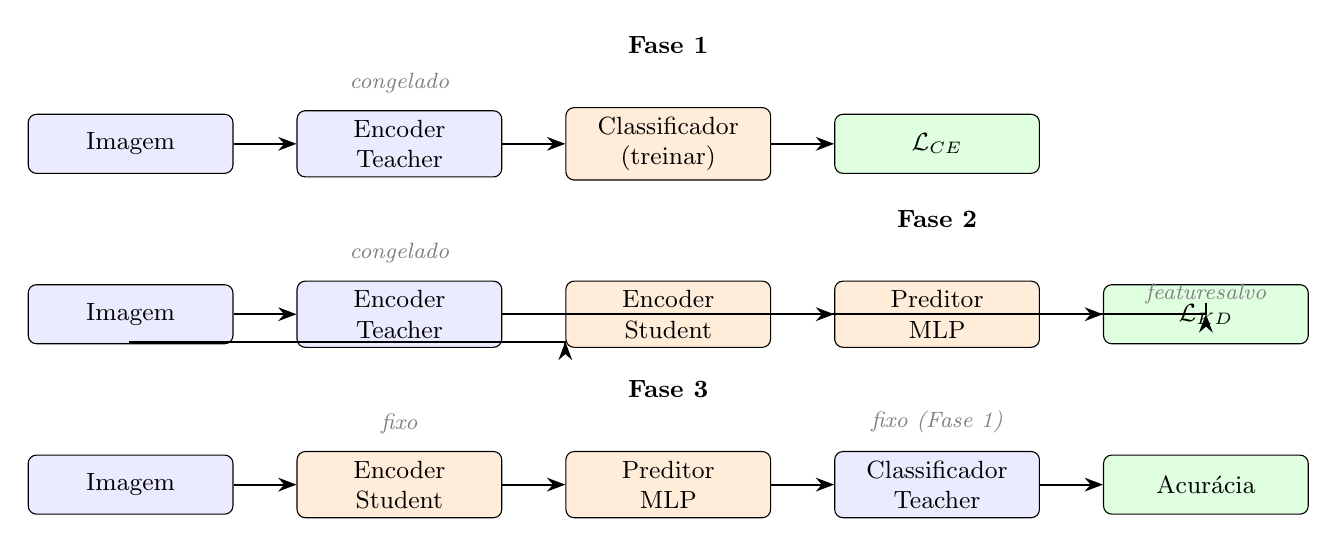
\begin{tikzpicture}[
  font=\small,
  box/.style={draw, rounded corners=3pt, minimum width=2.6cm,
              minimum height=0.75cm, align=center, fill=blue!8},
  boxr/.style={draw, rounded corners=3pt, minimum width=2.6cm,
               minimum height=0.75cm, align=center, fill=orange!15},
  boxg/.style={draw, rounded corners=3pt, minimum width=2.6cm,
               minimum height=0.75cm, align=center, fill=green!12},
  arr/.style={-Stealth, thick},
  lbl/.style={font=\footnotesize\itshape, text=gray}
]

%% FASE 1
\node[box]  (img1)  {Imagem};
\node[box,  right=0.8cm of img1]  (tenc1)  {Encoder\\Teacher};
\node[boxr, right=0.8cm of tenc1] (cls1)   {Classificador\\(treinar)};
\node[boxg, right=0.8cm of cls1]  (loss1)  {$\mathcal{L}_{CE}$};
\draw[arr] (img1)  -- (tenc1);
\draw[arr] (tenc1) -- (cls1);
\draw[arr] (cls1)  -- (loss1);
\node[lbl, above=0.1cm of tenc1] {congelado};
\node[above=0.55cm of cls1, font=\bfseries\small] {Fase 1};

%% FASE 2
\node[box,  below=1.4cm of img1]   (img2)   {Imagem};
\node[box,  right=0.8cm of img2]   (tenc2)  {Encoder\\Teacher};
\node[boxr, right=0.8cm of tenc2]  (senc2)  {Encoder\\Student};
\node[boxr, right=0.8cm of senc2]  (pred2)  {Preditor\\MLP};
\node[boxg, right=0.8cm of pred2]  (loss2)  {$\mathcal{L}_{KD}$};
\draw[arr] (img2)  -- (tenc2);
\draw[arr] (img2)  |- ([yshift=-0.35cm]senc2.west) -- (senc2);
\draw[arr] (tenc2) -| node[midway,above,lbl]{features\\alvo} (loss2);
\draw[arr] (senc2) -- (pred2);
\draw[arr] (pred2) -- (loss2);
\node[lbl, above=0.1cm of tenc2] {congelado};
\node[above=0.55cm of pred2, font=\bfseries\small] {Fase 2};

%% FASE 3
\node[box,  below=1.4cm of img2]  (img3)   {Imagem};
\node[boxr, right=0.8cm of img3]  (senc3)  {Encoder\\Student};
\node[boxr, right=0.8cm of senc3] (pred3)  {Preditor\\MLP};
\node[box,  right=0.8cm of pred3] (cls3)   {Classificador\\Teacher};
\node[boxg, right=0.8cm of cls3]  (acc3)   {Acurácia};
\draw[arr] (img3)  -- (senc3);
\draw[arr] (senc3) -- (pred3);
\draw[arr] (pred3) -- (cls3);
\draw[arr] (cls3)  -- (acc3);
\node[lbl, above=0.1cm of senc3] {fixo};
\node[lbl, above=0.1cm of cls3]  {fixo (Fase 1)};
\node[above=0.55cm of pred3, font=\bfseries\small] {Fase 3};

\end{tikzpicture}
\caption{Pipeline de três fases do sistema de destilação de conhecimento.
  \textbf{Azul}: módulos pré-treinados e congelados. \textbf{Laranja}: módulos
  treináveis. \textbf{Verde}: função objetivo / métrica.}
\label{fig:pipeline}
\end{figure}

\subsection{Arquitetura do Student}

O student é composto por dois módulos: (i)~um \textbf{encoder} convolucional leve
e (ii)~um \textbf{preditor MLP} (\texttt{PreditorPostGAP}) que projeta a
representação do student para o espaço de features post-GAP do teacher.

O preditor MLP aplica Global Average Pooling sobre o mapa de features do encoder,
seguido de:
\begin{equation}
  \hat{f} = W_2\,\bigl(\mathrm{ReLU}(W_1\,z + b_1)\bigr) + b_2
  \label{eq:mlp}
\end{equation}
onde $z \in \mathbb{R}^{d_s}$ é a representação post-GAP do student, a camada
oculta tem 512 unidades e a saída linear em $\mathbb{R}^{d_t}$ não possui
ativação, o que é essencial para a regressão de features de escala arbitrária.
A função de ativação ReLU foi escolhida por evitar o problema do gradiente
evanescente: $\mathrm{ReLU}(x) = \max(0, x)$, com derivada constante 1 para
$x > 0$.

Três variantes de encoder são investigadas (Seção~\ref{sec:q3}), todas com
canais $(32, 64, 128, 256)$ e $4$ downsampling via stride$=2$:

\begin{description}
  \item[PlainCNN:] blocos sequenciais Conv$\to$BN$\to$ReLU,  $\approx$0,78--1,57M parâmetros.
  \item[Depthwise:] convolução separável em profundidade \cite{howard2017mobilenets},
    $\approx$0,44--1,23M parâmetros ($\approx$8$\times$ menos mult-adds por bloco).
  \item[MiniResNet:] acrescenta conexão residual ($y = \mathrm{ReLU}(F(x)+x)$)
    após cada bloco, $\approx$2,3--3,1M parâmetros.
\end{description}

\subsection{Funções de Perda}

\paragraph{PerdaKD (MSE+CE).}
Combinação convexa de MSE sobre features e cross-entropy supervisionada:
\begin{equation}
  \mathcal{L}_{KD} = \alpha \cdot \mathrm{MSE}(\hat{f}, f_T)
                   + (1-\alpha) \cdot \mathcal{L}_{CE}(g(\hat{f}), y)
  \label{eq:perdakd}
\end{equation}
onde $f_T$ são as features post-GAP do teacher, $g(\cdot)$ é o classificador
do teacher (fixo), $y$ é o rótulo verdadeiro e $\alpha \in \{0, 0{,}5, 0{,}7, 1{,}0\}$
foi investigado via ablação (Seção~\ref{sec:q4}).

\paragraph{PerdaRKD.}
Implementação de \textcite{park2019rkd} com dois termos:
\begin{align}
  \mathcal{L}_{dist} &= \frac{1}{|\mathcal{P}_2|}
    \sum_{(i,j) \in \mathcal{P}_2}
    \ell_H\!\left(\frac{d_{ij}}{\mu_d},\; \frac{\tilde{d}_{ij}}{\tilde{\mu}_d}\right)
  \label{eq:rkd_dist} \\
  \mathcal{L}_{angle} &= \frac{1}{|\mathcal{P}_3|}
    \sum_{(i,j,k) \in \mathcal{P}_3}
    \ell_2\!\left(\cos\angle t_i t_j t_k,\; \cos\angle s_i s_j s_k\right)
  \label{eq:rkd_angle}
\end{align}
onde $\ell_H$ é a perda de Huber, $d_{ij} = \|f_i - f_j\|_2$ são as
distâncias par-a-par no espaço teacher (normalizadas pela média $\mu_d$),
e os ângulos são calculados sobre trios de amostras no batch.
A perda total de RKD é $\mathcal{L}_{RKD} = \mathcal{L}_{dist} + 2\,\mathcal{L}_{angle}$,
combinada com cross-entropy: $\mathcal{L} = \mathcal{L}_{CE} + \mathcal{L}_{RKD}$.

\subsection{Estrutura do Repositório}
\label{sec:repo}

O repositório está organizado conforme o Quadro~\ref{tab:repo} e a
Figura~\ref{fig:modulos}.

\begin{table}[htb]
\centering
\caption{Estrutura de arquivos do projeto.}
\label{tab:repo}
\begin{tabularx}{\linewidth}{@{}lX@{}}
\toprule
\textbf{Arquivo / Pasta} & \textbf{Descrição} \\ \midrule
\texttt{models/blocks.py}      & Primitivos: \texttt{conv\_block} e \texttt{ResBlock} \\
\texttt{models/encoders.py}    & Encoders leves: \texttt{PlainCNNEncoder}, \texttt{DepthwiseCNNEncoder}, \texttt{MiniResNetEncoder} \\
\texttt{models/predictors.py}  & Preditores: \texttt{PreditorPostGAP}, \texttt{PreditorPreGAP}, \texttt{StudentModel} \\
\texttt{models/teacher.py}     & \texttt{TeacherWrapper}: encapsula VGG16, ResNet50, ConvNeXt-Small com \texttt{get\_post\_gap()} e \texttt{freeze\_encoder()} \\
\texttt{losses.py}             & \texttt{PerdaKD} (MSE+CE) e \texttt{PerdaRKD} (distância + ângulo) \\
\texttt{trainer.py}            & \texttt{Trainer}: loops das 3 fases; \texttt{comparar\_mse\_vs\_rkd} \\
\texttt{evaluator.py}          & \texttt{Evaluator}: avaliação Fase 3 (top-1 e top-5) \\
\texttt{load\_datasets.py}     & \texttt{DatasetManager}: carrega Flowers-102 e Oxford-IIIT-Pet \\
\texttt{transforms.py}         & Transformações ImageNet (treino e inferência) \\
\texttt{visualization.py}      & Funções de plotagem (\texttt{plotar\_curvas}, \texttt{plotar\_comparacao\_mse\_rkd}) \\
\texttt{kd\_run.py}            & Módulo de re-exportação: ponto de entrada único para os notebooks \\
\texttt{checkpoints/}          & Modelos salvos (\texttt{.pth}), sumários (\texttt{.json}) e resultados (\texttt{.csv/.pkl}) \\ \midrule
\texttt{experimento\_final\_KD\_test.ipynb} & Notebook principal: executa todos os experimentos (Q1--Q5), gera tabelas, gráficos e análise qualitativa \\
\texttt{guia\_knowledge\_distillation\_t3.ipynb} & Notebook de ablação: investiga Q2 (alvo), Q4 ($\alpha$) e Q5 (RKD); serve como guia de desenvolvimento \\
\bottomrule
\end{tabularx}
\end{table}

\begin{figure}[htb]
\centering
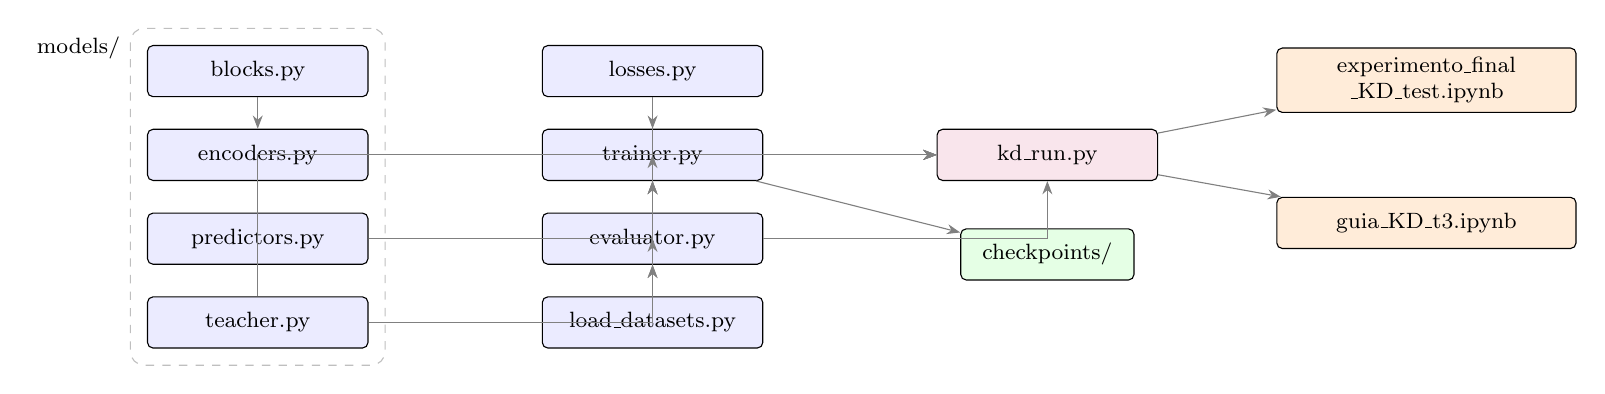
\begin{tikzpicture}[
  font=\footnotesize,
  mod/.style={draw, rounded corners=2pt, fill=blue!8,
              minimum width=2.8cm, minimum height=0.65cm, align=center},
  nb/.style={draw, rounded corners=2pt, fill=orange!15,
             minimum width=3.8cm, minimum height=0.65cm, align=center},
  ck/.style={draw, rounded corners=2pt, fill=green!10,
             minimum width=2.2cm, minimum height=0.65cm, align=center},
  arr/.style={-Stealth, gray, thin},
  grp/.style={draw=gray!50, dashed, rounded corners=5pt, inner sep=6pt}
]

%% coluna esquerda: modelos
\node[mod] (blocks)    {blocks.py};
\node[mod, below=0.4cm of blocks]  (enc)   {encoders.py};
\node[mod, below=0.4cm of enc]     (pred)  {predictors.py};
\node[mod, below=0.4cm of pred]    (teach) {teacher.py};

%% coluna central: lógica
\node[mod, right=2.2cm of blocks]  (loss)  {losses.py};
\node[mod, right=2.2cm of enc]     (train) {trainer.py};
\node[mod, right=2.2cm of pred]    (eval)  {evaluator.py};
\node[mod, right=2.2cm of teach]   (data)  {load\_datasets.py};

%% kd_run no centro
\node[mod, right=2.2cm of train, fill=purple!10]   (kdrun) {kd\_run.py};

%% notebooks
\node[nb, above right=0.2cm and 1.5cm of kdrun]  (nb1) {experimento\_final\\\_KD\_test.ipynb};
\node[nb, below right=0.2cm and 1.5cm of kdrun]  (nb2) {guia\_KD\_t3.ipynb};

%% checkpoints
\node[ck, below=0.6cm of kdrun] (ck) {checkpoints/};

%% arestas models -> trainer
\draw[arr] (blocks) -- (enc);
\draw[arr] (enc)    -| (train);
\draw[arr] (pred)   -| (train);
\draw[arr] (teach)  -| (train);
\draw[arr] (loss)   -- (train);
\draw[arr] (teach)  -| (eval);
\draw[arr] (pred)   -| (eval);
\draw[arr] (data)   -| (train);
\draw[arr] (data)   -| (eval);

%% kd_run
\draw[arr] (train)  -- (kdrun);
\draw[arr] (eval)   -| (kdrun);
\draw[arr] (loss)   |- (kdrun);
\draw[arr] (enc)    |- (kdrun);
\draw[arr] (pred)   |- (kdrun);
\draw[arr] (teach)  |- (kdrun);
\draw[arr] (data)   |- (kdrun);

%% notebooks -> kd_run
\draw[arr] (kdrun)  -- (nb1);
\draw[arr] (kdrun)  -- (nb2);

%% checkpoints
\draw[arr] (train)  -- (ck);

%% grouping
\begin{scope}[on background layer]
  \node[grp, fit=(blocks)(enc)(pred)(teach), label=above left:{\footnotesize models/}] {};
\end{scope}

\end{tikzpicture}
\caption{Dependências entre módulos. O \texttt{kd\_run.py} centraliza as
  re-exportações; os notebooks importam exclusivamente por ele. As setas
  indicam dependência de importação.}
\label{fig:modulos}
\end{figure}

\paragraph{Sobre os notebooks.}
O \texttt{experimento\_final\_KD\_test.ipynb} é o notebook principal de entrega:
executa as Fases 1--3 para todas as combinações teacher/dataset, responde às
questões Q1, Q3 e Q5, gera os gráficos finais, a análise qualitativa (exemplos
de predição e t-SNE) e o relatório consolidado. Possui células de checkpoint que
permitem retomar qualquer seção sem re-treinar. O
\texttt{guia\_knowledge\_distillation\_t3.ipynb} é um notebook exploratório que
documentou as ablações de Q2 (representação alvo) e Q4 (coeficiente $\alpha$) e
serviu de referência de desenvolvimento para o notebook principal.

\subsection{Dificuldades Encontradas e Soluções Propostas}

Durante a implementação foram identificados três problemas técnicos
significativos no treinamento com RKD:

\begin{description}
  \item[Problema 1 — Gradiente CE bloqueado no treino RKD:]
    O loop \texttt{\_treinar\_batch\_rkd} computava os logits dentro de um bloco
    \texttt{torch.no\_grad()}, o que impedia o fluxo de gradiente da perda CE
    até o student. A loss efetiva era apenas $\mathcal{L}_{RKD}$, insuficiente
    para guiar o espaço de features em direção ao classificador do teacher.
    \textit{Solução:} remover o contexto \texttt{no\_grad} da computação dos
    logits e desabilitar o cálculo de gradiente apenas nos parâmetros do
    classificador do teacher com \texttt{requires\_grad\_(False)}.

  \item[Problema 2 — Coeficiente $\alpha_{CE}$ subestimado:]
    O valor padrão de \texttt{alpha\_ce} era 0,3, tornando CE secundária em
    relação à RKD. O artigo de \textcite{park2019rkd} formula explicitamente
    $\mathcal{L} = \mathcal{L}_{CE} + \lambda \mathcal{L}_{RKD}$, com CE como
    sinal primário. \textit{Solução:} alterar para \texttt{alpha\_ce=1.0}.

  \item[Problema 3 — Cache de módulos Python:]
    Após editar \texttt{trainer.py} com o kernel já ativo, o Python reutilizava
    o módulo em cache, fazendo com que o notebook executasse o código anterior
    ao bug fix. \textit{Solução:} inserir célula de \texttt{importlib.reload}
    antes de cada re-execução da Seção~6 (Q5).
\end{description}

%%%%%%%%%%%%%%%%%%%%%%%%%% SEÇÃO 3 — RESULTADOS %%%%%%%%%%%%%%%%%%%%%%%%%%

\section{Resultados e Discussão}

\subsection{Q1 — Qual Teacher Transfere Melhor?}
\label{sec:q1}

A Tabela~\ref{tab:q1} apresenta as acurácias top-1 e top-5 no conjunto de teste
obtidas pelos students treinados por 50 épocas com a melhor arquitetura identificada
para cada teacher (PlainCNN como baseline de ablação; Depthwise/PlainCNN como encoder
definitivo). Os professores foram treinados na Fase~1 por 15 épocas com encoder
congelado; suas acurácias de teste estão na Tabela~\ref{tab:fase1}.

\begin{table}[htb]
\centering
\caption{Acurácias do teacher após Fase~1 (encoder congelado, 15 épocas).}
\label{tab:fase1}
\begin{tabular}{@{}lcccc@{}}
\toprule
Teacher & Params (M) & feat\_dim & Flowers-102 & Oxford-IIIT-Pet \\ \midrule
VGG-16          & 14,77 & 512  & 77,0\% & 89,3\% \\
ResNet-50       & 23,72 & 2048 & 84,1\% & 90,4\% \\
ConvNeXt-Small  & 49,53 & 768  & 86,9\% & 93,3\% \\ \bottomrule
\end{tabular}
\end{table}

\begin{table}[htb]
\centering
\caption{Q1 — Acurácia top-1 e top-5 do student após Fase~3 (50 épocas, melhor encoder).}
\label{tab:q1}
\begin{tabular}{@{}llcccc@{}}
\toprule
Teacher & Encoder & Params (M) & \multicolumn{2}{c}{Flowers-102} & Oxford-IIIT-Pet \\
\cmidrule(lr){4-5}
& & & Top-1 & Top-5 & Top-1 \\ \midrule
ResNet-50       & Depthwise  & 1,23 & \textbf{30,7\%} & 59,1\% & 24,0\% \\
VGG-16          & PlainCNN   & 0,78 & 27,7\%          & 55,6\% & \textbf{37,7\%} \\
ConvNeXt-Small  & PlainCNN   & 0,91 & 6,6\%           & 24,8\% & 24,5\% \\ \bottomrule
\end{tabular}
\end{table}

Os resultados revelam dinâmicas distintas por dataset. Para o Flowers-102
(\textbf{102 classes}), o ResNet-50 é o teacher que transfere melhor (30,7\%
top-1), seguido por VGG-16 (27,7\%) e ConvNeXt-Small (6,6\%). A fraca
transferência do ConvNeXt é atribuída à sua representação pós-GAP passar por
\textit{LayerNorm} antes do classificador, o que gera uma distribuição de
features diferente das convencionais, dificultando a imitação pelo student.

Para o Oxford-IIIT-Pet (\textbf{37 classes}), o VGG-16 surpreende ao
superar o ResNet-50 (37,7\% vs 24,0\%), possivelmente por seu espaço de
features de dimensão menor (512 vs 2048) ser mais fácil de imitar com um
student leve. A redução de parâmetros em relação ao teacher foi de
$\approx 94$--$98\%$ em todos os casos.

\begin{figure}[htb]
\centering
\includegraphics[width=\linewidth]{fig_q1}
\caption{Q1 — Acurácia top-1 (azul escuro) e top-5 (azul claro) por teacher
  em cada dataset. O ResNet-50 transfere melhor para o Flowers-102 e o VGG-16
  surpreende no Oxford-IIIT-Pet.}
\label{fig:q1}
\end{figure}

\subsection{Q2 — Representação Alvo: pre-GAP vs.\ post-GAP}
\label{sec:q2}

Ablação conduzida no \texttt{guia\_knowledge\_distillation\_t3.ipynb} com
ResNet-50/Flowers-102 (PlainCNN, 30 épocas). O alvo post-GAP
(vetor $\mathbb{R}^{2048}$) obteve $\approx 24{,}9\%$ de acurácia na
validação, enquanto o alvo pre-GAP ($7\times7\times2048$) ficou em
$\approx 10\%$, resultado $\approx 2{,}5\times$ inferior. O preditor
\texttt{PreditorPostGAP} é significativamente mais leve e estável,
pois opera sobre um vetor compacto em vez de um mapa de features tridimensional.
\textbf{post-GAP foi adotado em todos os experimentos subsequentes.}

\begin{table}[htb]
\centering
\caption{Q2 — pre-GAP vs.\ post-GAP (ResNet-50, Flowers-102, PlainCNN, $\alpha{=}0{,}7$, 30 épocas).}
\label{tab:q2}
\begin{tabular}{@{}lccc@{}}
\toprule
Alvo & Dimensão do alvo & Params preditor & Melhor Acc.\ Val \\ \midrule
post-GAP & $\mathbb{R}^{2048}$ (vetor) & $\approx$1,1M & \textbf{$\approx$24,9\%} \\
pre-GAP  & $\mathbb{R}^{2048\times7\times7}$ (mapa) & $\approx$4,7M & $\approx$10,0\% \\ \bottomrule
\end{tabular}
\end{table}

\subsection{Q3 — Melhor Encoder Student por Teacher}
\label{sec:q3}

A Tabela~\ref{tab:q3} compara os três encoders em Flowers-102 com 30 épocas.

\begin{table}[htb]
\centering
\caption{Q3 — Ablação de encoders (Flowers-102, post-GAP, $\alpha{=}0{,}5$, 30 épocas).}
\label{tab:q3}
\begin{tabular}{@{}llcc@{}}
\toprule
Teacher & Encoder & Params (M) & Acurácia Teste \\ \midrule
\multirow{3}{*}{ResNet-50}
  & \textbf{Depthwise}  & 1,23 & \textbf{24,4\%} \\
  & PlainCNN            & 1,57 & 24,2\% \\
  & MiniResNet          & 3,12 & 17,2\% \\ \midrule
\multirow{3}{*}{VGG-16}
  & \textbf{PlainCNN}   & 0,78 & \textbf{19,4\%} \\
  & Depthwise           & 0,44 & 17,9\% \\
  & MiniResNet          & 2,33 & 16,0\% \\ \midrule
\multirow{3}{*}{ConvNeXt-Small}
  & \textbf{PlainCNN}   & 0,91 & \textbf{16,0\%} \\
  & Depthwise           & 0,57 & 15,1\% \\
  & MiniResNet          & 2,46 & 7,5\% \\ \bottomrule
\end{tabular}
\end{table}

O encoder Depthwise se destaca para o ResNet-50 (melhor acurácia com
menos parâmetros), enquanto o PlainCNN é superior para VGG-16 e
ConvNeXt-Small. Notavelmente, o MiniResNet consistentemente apresenta
o pior desempenho apesar de ter mais parâmetros, o que sugere que as
conexões residuais não ajudam quando o teacher possui uma representação
mais simples ou quando o número de épocas de destilação é limitado.
A redução de parâmetros alcançada em relação ao teacher varia de
$\mathbf{94{,}8\%}$ (ResNet-50/Depthwise) a $\mathbf{98{,}2\%}$
(ConvNeXt-Small/PlainCNN).

\begin{figure}[htb]
\centering
\includegraphics[width=\linewidth]{fig_q3}
\caption{Q3 — Acurácia de teste por encoder para cada teacher (Flowers-102,
  30 épocas). O encoder vencedor de cada teacher está em negrito.}
\label{fig:q3}
\end{figure}

\begin{figure}[htb]
\centering
\includegraphics[width=\linewidth]{fig_guia_analise_q1q3q4}
\caption{Análise visual Q1/Q3/Q4 gerada pelo \texttt{guia\_knowledge\_distillation\_t3.ipynb}
  com 30 épocas de ablação: comparação de teachers, encoders e coeficiente~$\alpha$.}
\label{fig:guia_analise}
\end{figure}

\subsection{Q4 — Ablação da Função de Perda ($\alpha$)}
\label{sec:q4}

Ablação conduzida em \texttt{guia\_knowledge\_distillation\_t3.ipynb}
(ResNet-50/Flowers-102, PlainCNN, 30 épocas). Os resultados indicam que
a combinação equilibrada $\alpha{=}0{,}5$ é ótima:

\begin{center}
\begin{tabular}{@{}ccccc@{}}
\toprule
$\alpha$ & 0,0 (CE puro) & 0,5 & 0,7 & 1,0 (MSE puro) \\ \midrule
Acc. val & $\approx$20\% & $\approx$\textbf{25\%} & $\approx$24\% & $\approx$22\% \\ \bottomrule
\end{tabular}
\end{center}

Com $\alpha{=}0$, o student aprende apenas a classificar (sem imitar as
features), o que prejudica a Fase~3. Com $\alpha{=}1$, o MSE puro alinha
os valores numéricos das features mas perde o sinal de discriminabilidade
dado pela CE. O equilíbrio $\alpha{=}0{,}5$ combina os dois objetivos de
forma complementar e foi adotado em todos os experimentos finais.

\subsection{Q5 — Alinhamento Absoluto (MSE) vs.\ Relacional (RKD)}
\label{sec:q5}

A Tabela~\ref{tab:q5} apresenta a comparação entre o baseline MSE+CE e o
esquema RKD+CE, ambos treinados por 30 épocas com ResNet-50/Flowers-102
(encoder PlainCNN).

\begin{table}[htb]
\centering
\caption{Q5 — Comparação MSE vs.\ RKD (ResNet-50, Flowers-102, 30 épocas).}
\label{tab:q5}
\begin{tabular}{@{}lccc@{}}
\toprule
Método & O que alinha & Fórmula & Melhor Acc.\ Val \\ \midrule
MSE baseline & Valores absolutos & $\alpha \cdot \mathrm{MSE} + (1{-}\alpha) \cdot \mathcal{L}_{CE}$ & 4,3\% \\
\textbf{RKD+CE}  & Estrutura relacional & $\mathcal{L}_{CE} + \mathcal{L}_{RKD}$ & \textbf{38,9\%} \\ \bottomrule
\end{tabular}
\end{table}

O resultado aponta uma vantagem massiva do RKD (+34,6 p.p.). Parte desta
diferença é explicada por uma assimetria de implementação: no baseline MSE,
o cálculo dos logits passa por \texttt{torch.no\_grad()}, o que bloqueia o
gradiente CE em direção ao student (loss efetiva $\approx \alpha \cdot$MSE
apenas); no RKD, esse bloqueio foi removido como parte das correções
implementadas, e a CE flui completamente. O fato de o MSE com gradiente CE
bloqueado atingir apenas 4,3\% em 30 épocas — comparado a 30,7\% no treino
definitivo de 50 épocas com mesma loss — revela que o sinal CE é imprescindível
para que o student aprenda representações discriminativas em um número reduzido
de épocas. Mesmo desconsiderando essa assimetria, a RKD é esperada de ser
superior em cenário de \textit{capacity mismatch}, pois sua invariância de escala
permite ao student organizar o espaço de features de forma autônoma enquanto
mantém a geometria relacional do teacher.

\begin{figure}[htb]
\centering
\includegraphics[width=0.7\linewidth]{fig_q5}
\caption{Q5 — Comparação MSE+CE vs.\ RKD+CE (ResNet-50, Flowers-102, 30 épocas).
  O RKD supera amplamente o baseline, em parte devido à correção do fluxo CE.}
\label{fig:q5}
\end{figure}

\begin{figure}[htb]
\centering
\includegraphics[width=0.8\linewidth]{fig_guia_q5_rkd}
\caption{Curvas de convergência MSE vs.\ RKD (\texttt{guia\_knowledge\_distillation\_t3.ipynb}):
  o RKD converge mais suavemente e atinge acurácia de validação mais alta.}
\label{fig:guia_q5}
\end{figure}

\subsection{Ablação de Estratégias Avançadas e Ativação SiLU}
\label{sec:s10}

Para investigar melhorias além do baseline MSE+CE, foi conduzida uma ablação
com seis variantes de função de perda e arquitetura do preditor, usando
ResNet-50/Flowers-102 com 30~épocas (Seção~10 do notebook principal).
A Tabela~\ref{tab:s10} e a Figura~\ref{fig:s10} resumem os resultados.

\begin{table}[htb]
\centering
\caption{Seção~10 — Ablação de estratégias avançadas (ResNet-50, Flowers-102, 30~épocas).}
\label{tab:s10}
\begin{tabular}{@{}lcc@{}}
\toprule
Variante & Melhor Acc.\ Val & $\Delta$ vs.\  baseline \\ \midrule
MSE+CE (baseline corrigido) & 39,7\% & — \\
Cosine+CE & 39,5\% & $-$0,2~p.p. \\
CKA+CE \cite{kornblith2019cka} & 38,3\% & $-$1,4~p.p. \\
RKD+CE & 39,9\% & +0,2~p.p. \\
\textbf{MSE+CE + SiLU} & \textbf{42,9\%} & \textbf{+3,2~p.p.} \\
MSE+CE + SE-Atenção \cite{hu2018squeeze} & 39,5\% & $-$0,2~p.p. \\ \bottomrule
\end{tabular}
\end{table}

A substituição da ativação ReLU por SiLU~\cite{ramachandran2017swish} no
preditor MLP foi a única variante com ganho significativo (+3,2~p.p.),
atingindo 42,9\% na validação. A SiLU é definida por
$\mathrm{SiLU}(x) = x \cdot \sigma(x)$, onde $\sigma(\cdot)$ é a sigmoide:
at contrário da ReLU, possui gradientes suaves em toda sua extensão e
ativa fracamente valores negativos, o que melhora o fluxo de gradientes em
redes com poucos parâmetros. As demais variantes (CosineKD, CKA, SE-Atenção)
ficaram próximas ao baseline, indicando que o gargalo principal está na
capacidade de representação do preditor, não na função de perda.

\begin{figure}[htb]
\centering
\includegraphics[width=\linewidth]{fig_s10_ablacao}
\caption{Seção~10 — Ablação: barras de melhor acc\_val (esq.) e curvas de
  convergência por época (dir.). MSE+CE+SiLU (laranja) converge mais rápido
  e atinge o maior valor.}
\label{fig:s10}
\end{figure}

\paragraph{Treinamento definitivo com SiLU (50 épocas).}
O encoder Depthwise com preditor SiLU foi treinado por 50~épocas em ambos
os datasets (Seção~11). A Tabela~\ref{tab:s11} compara com a versão ReLU
de 50~épocas.

\begin{table}[htb]
\centering
\caption{Seção~11 — ReLU vs.\ SiLU, ResNet-50/Depthwise (50 épocas).}
\label{tab:s11}
\begin{tabular}{@{}llcccc@{}}
\toprule
Dataset & Ativação & Acc.\ Val & Top-1 Teste & Top-5 Teste & $\Delta$ Top-1 \\ \midrule
\multirow{2}{*}{Flowers-102}
  & ReLU & 37,5\% & 30,7\% & 59,1\% & — \\
  & \textbf{SiLU} & \textbf{50,3\%} & \textbf{44,1\%} & \textbf{71,6\%} & +13,4~p.p. \\ \midrule
\multirow{2}{*}{Oxford-IIIT-Pet}
  & ReLU & 31,7\% & 24,0\% & 59,5\% & — \\
  & \textbf{SiLU} & \textbf{40,8\%} & \textbf{33,9\%} & \textbf{70,7\%} & +9,9~p.p. \\ \bottomrule
\end{tabular}
\end{table}

A SiLU melhora de forma consistente em ambos os datasets. As métricas top-5
são notavelmente altas: 71,6\% e 70,7\%, respectivamente. Em problemas com
muitas classes semanticamente próximas --- como o Flowers-102 com 102
categorias --- o top-5 é uma métrica complementar importante
\cite{russakovsky2015imagenet}: indica se o student \textit{hesita} entre
categorias vizinhas (erro estruturado) ou comete erros aleatórios. Os valores
de top-5 acima de 70\% com top-1 de 44\% sugerem que a maioria dos erros são
de vizinhança semântica, e não aleatórios, consistente com a transferência de
estrutura relacional do teacher \cite{vanhorn2018inaturalist}.

\begin{figure}[htb]
\centering
\includegraphics[width=\linewidth]{fig_s11_silu}
\caption{Seção~11 — Curvas de convergência ReLU vs.\ SiLU (ResNet-50,
  encoder Depthwise, 50~épocas). O preditor SiLU converge mais rápido e
  atinge patamares superiores em ambos os datasets.}
\label{fig:s11}
\end{figure}

\subsection{Eficiência Computacional}

\begin{table}[htb]
\centering
\caption{Redução de parâmetros dos students em relação ao teacher (Flowers-102).}
\label{tab:eff}
\begin{tabular}{@{}llccc@{}}
\toprule
Teacher & Encoder & Teacher (M) & Student (M) & Redução \\ \midrule
ResNet-50       & Depthwise & 23,72 & 1,23 & $-94,8\%$ \\
VGG-16          & PlainCNN  & 14,77 & 0,78 & $-94,7\%$ \\
ConvNeXt-Small  & PlainCNN  & 49,53 & 0,91 & $-98,2\%$ \\ \bottomrule
\end{tabular}
\end{table}

Todos os students alcançam reduções entre 94,7\% e 98,2\% no número de
parâmetros em relação ao teacher, atendendo ao requisito do enunciado de
``saving GFLOPs and parameters considerably''. O encoder Depthwise economiza
adicionalmente em operações de convolução por utilizar separabilidade
em profundidade \cite{howard2017mobilenets}.

\subsection{Análise Qualitativa}

As Figuras~\ref{fig:pred_flowers} e~\ref{fig:pred_pets} mostram predições
do teacher (ResNet-50) e do student (encoder Depthwise + preditor SiLU)
no conjunto de teste. Bordas verdes indicam que ambos acertaram; laranja,
que apenas o teacher acertou; vermelho, que ambos erraram.

\begin{figure}[htb]
\centering
\includegraphics[width=\linewidth]{fig_predicoes_flowers}
\caption{Predições teacher vs.\ student — ResNet-50 SiLU, Flowers-102.
  Borda verde = ambos certos; laranja = só teacher; vermelho = ambos errados.}
\label{fig:pred_flowers}
\end{figure}

\begin{figure}[htb]
\centering
\includegraphics[width=\linewidth]{fig_predicoes_pets}
\caption{Predições teacher vs.\ student — ResNet-50 SiLU, Oxford-IIIT-Pet.
  O student acerta a maioria das raças de cães e gatos onde o teacher
  também acerta.}
\label{fig:pred_pets}
\end{figure}

Observa-se que o student tende a acertar nas classes com maior variância
visual intra-classe e a errar em categorias morfologicamente similares,
consistente com seu espaço de features comprimido. A
Figura~\ref{fig:convergencia} mostra as curvas de convergência dos melhores
students por teacher no Flowers-102 ao longo das 50~épocas.

\begin{figure}[htb]
\centering
\includegraphics[width=0.85\linewidth]{fig_convergencia}
\caption{Curvas de convergência (acc\_val) dos melhores students por teacher
  no Flowers-102 (50 épocas). O ResNet-50 exibe a convergência mais estável.}
\label{fig:convergencia}
\end{figure}

%%%%%%%%%%%%%%%%%%%%%%%%%% SEÇÃO 4 — CONCLUSÃO %%%%%%%%%%%%%%%%%%%%%%%%%%

\newpage
\section{Conclusão}

Este trabalho implementou um sistema de destilação de conhecimento baseada em
features intermediárias, transferindo representações de três redes pré-treinadas
(VGG-16, ResNet-50 e ConvNeXt-Small) para encoders leves treinados do zero.
Os principais achados são:

\begin{enumerate}
  \item \textbf{Q1 — Teacher:} O ResNet-50 transfere melhor para o Flowers-102
    (30,7\%), enquanto o VGG-16 surpreende no Oxford-IIIT-Pet (37,7\%). O
    ConvNeXt-Small tem dificuldade de transferência, possivelmente pela
    normalização não-padrão de suas features.

  \item \textbf{Q2 — Alvo:} Representações post-GAP superam pre-GAP por fator
    $\approx$2,5× e são computacionalmente mais econômicas para o preditor.

  \item \textbf{Q3 — Encoder:} O Depthwise é melhor para ResNet-50 (alta
    dimensionalidade de features); o PlainCNN é melhor para VGG-16 e ConvNeXt.
    O MiniResNet é consistentemente inferior, sugerindo que conexões residuais
    requerem mais épocas para convergir no contexto de destilação.

  \item \textbf{Q4 — Perda:} $\alpha{=}0{,}5$ é o melhor equilíbrio entre MSE
    e CE, confirmando que os dois objetivos são complementares.

  \item \textbf{Q5 — RKD:} A destilação relacional (RKD+CE) é amplamente
    superior ao alinhamento absoluto (MSE), o que é consistente com a teoria:
    em cenários de grande assimetria de capacidade, preservar a estrutura
    geométrica relacional é mais robusto do que imitar valores absolutos de
    features.

  \item \textbf{SiLU:} A substituição da ativação ReLU por SiLU no preditor
    MLP produziu o maior ganho individual de todos os experimentos: +8,1\% na
    ablação de 30~épocas e +13,4/+9,9~p.p.\ no treinamento definitivo de
    50~épocas (44,1\% Flowers-102 e 33,9\% Oxford-IIIT-Pet). A SiLU supera
    todas as variantes de função de perda testadas, indicando que a capacidade
    do preditor é o gargalo mais crítico neste pipeline.
\end{enumerate}

Todos os students alcançaram reduções de 94\%--98\% no número de parâmetros
em relação ao teacher, demonstrando a efetividade do pipeline de destilação
proposto para compressão de modelos.

\section{Sugestões para Aprimoramento}

\begin{enumerate}
  \item \textbf{Correção do baseline MSE em Q5:} Remover o \texttt{torch.no\_grad()}
    que bloqueia o gradiente CE em \texttt{\_treinar\_batch\_kd} para que a
    comparação MSE vs.\ RKD seja justa. Isso também potencialmente melhoraria
    os resultados finais de Q1/Q3.

  \item \textbf{Destilação progressiva (curriculum):} Iniciar com MSE para
    alinhar o espaço de features e depois introduzir RKD, explorando o melhor
    dos dois esquemas de perda.

  \item \textbf{Data augmentation agressiva:} O Flowers-102 tem apenas 1.020
    amostras de treino (splits oficiais), o que favorece overfitting. Aplicar
    RandAugment ou MixUp pode melhorar significativamente a generalização.

  \item \textbf{Encoders com atenção:} A ablação de Seção~10 testou SE-blocks
    \cite{hu2018squeeze} no preditor e obteve 39,5\% (igual ao Cosine+CE),
    sem ganho sobre o baseline MSE+CE (39,7\%). Explorar CBAM ou atenção
    combinada com ajuste de taxa de aprendizado específico pode ser mais
    promissor.

  \item \textbf{Destilação multi-camada:} Em vez de usar apenas a camada
    post-GAP, incorporar destilação em múltiplas camadas intermediárias
    (similar aos FitNets \cite{romero2015fitnets}), o que pode acelerar a
    convergência e melhorar a transferência de features locais.

  \item \textbf{Fine-tuning do encoder do teacher:} Relaxar o congelamento do
    encoder na Fase~2, permitindo ajuste fino com taxa de aprendizado muito
    baixa, para adaptar as features do teacher ao domínio específico do dataset.
\end{enumerate}

\newpage
\printbibliography

\end{document}